\begin{figure}[!h]
    \centering
    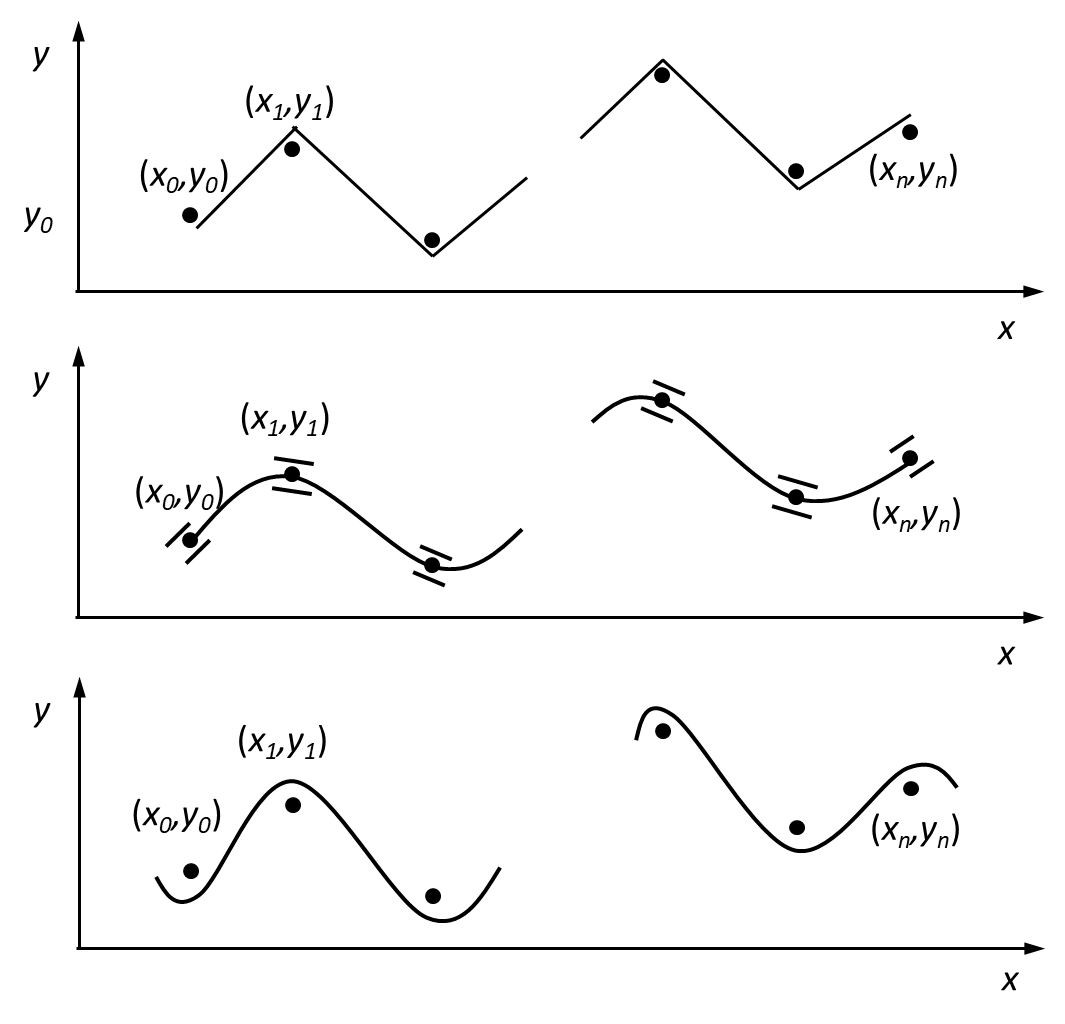
\includegraphics[width=.8\textwidth]{figures/phys_spline.png}
    \caption{сверху-вниз: 
    линейный сплайн с дефектом 1; 
    сплайн степени 3 с дефектом 2;
    сплайн степени 3 с дефектом 1
    }
\end{figure}

Линейный сплайн может быть проинтерпретирован, как уравнение нитки, туго натянутой на гвоздики на стене. Сплайн степени 3 с дефектом 2 может быть представлен, как уравнение упругой линейки, которая продета через желобки, у которых задана ориентация. Сплайн степени 3 с дефектом 1 может также соответствовать упругой линейке, которая проходит между гвоздиками, направление которых невозможно определить.

Причем интересным фактом является то, что уравнение свободного равновесия гибкого упругого бруска $\phi^{IV}(x) = 0$ соответствует \eqref{Eq:spline_3}.